\documentclass[11pt,compress,t,notes=noshow, xcolor=table]{beamer}
\usepackage[]{graphicx}\usepackage[]{color}
% maxwidth is the original width if it is less than linewidth
% otherwise use linewidth (to make sure the graphics do not exceed the margin)
\makeatletter
\def\maxwidth{ %
  \ifdim\Gin@nat@width>\linewidth
    \linewidth
  \else
    \Gin@nat@width
  \fi
}
\makeatother

\newcommand{\citebutton}[2]{%
\beamergotobutton{\href{#2}{#1}}%
}

\newcommand{\blu}[1]{\textcolor{blue}{#1}}
\newcommand{\org}[1]{\textcolor{orange}{#1}}
\newcommand{\ques}{\textbf{\textcolor{red}{Question:  }}}
\newcommand{\questionssofar}{\begin{frame}\frametitle{Any questions?}\end{frame}}

\newcommand\warning{%
 \makebox[1.4em][c]{%
 \makebox[0pt][c]{\raisebox{.1em}{\scriptsize!}}%
 \makebox[0pt][c]{\color{red}\normalsize$\bigtriangleup$}}}%

\definecolor{fgcolor}{rgb}{0.345, 0.345, 0.345}
\newcommand{\hlnum}[1]{\textcolor[rgb]{0.686,0.059,0.569}{#1}}%
\newcommand{\hlstr}[1]{\textcolor[rgb]{0.192,0.494,0.8}{#1}}%
\newcommand{\hlcom}[1]{\textcolor[rgb]{0.678,0.584,0.686}{\textit{#1}}}%
\newcommand{\hlopt}[1]{\textcolor[rgb]{0,0,0}{#1}}%
\newcommand{\hlstd}[1]{\textcolor[rgb]{0.345,0.345,0.345}{#1}}%
\newcommand{\hlkwa}[1]{\textcolor[rgb]{0.161,0.373,0.58}{\textbf{#1}}}%
\newcommand{\hlkwb}[1]{\textcolor[rgb]{0.69,0.353,0.396}{#1}}%
\newcommand{\hlkwc}[1]{\textcolor[rgb]{0.333,0.667,0.333}{#1}}%
\newcommand{\hlkwd}[1]{\textcolor[rgb]{0.737,0.353,0.396}{\textbf{#1}}}%
\let\hlipl\hlkwb

\usepackage{framed}
\makeatletter
\newenvironment{kframe}{%
 \def\at@end@of@kframe{}%
 \ifinner\ifhmode%
  \def\at@end@of@kframe{\end{minipage}}%
  \begin{minipage}{\columnwidth}%
 \fi\fi%
 \def\FrameCommand##1{\hskip\@totalleftmargin \hskip-\fboxsep
 \colorbox{shadecolor}{##1}\hskip-\fboxsep
     % There is no \\@totalrightmargin, so:
     \hskip-\linewidth \hskip-\@totalleftmargin \hskip\columnwidth}%
 \MakeFramed {\advance\hsize-\width
   \@totalleftmargin\z@ \linewidth\hsize
   \@setminipage}}%
 {\par\unskip\endMakeFramed%
 \at@end@of@kframe}
\makeatother

\definecolor{shadecolor}{rgb}{.97, .97, .97}
\definecolor{messagecolor}{rgb}{0, 0, 0}
\definecolor{warningcolor}{rgb}{1, 0, 1}
\definecolor{errorcolor}{rgb}{1, 0, 0}
\newenvironment{knitrout}{}{} % an empty environment to be redefined in TeX

\usepackage{alltt}
\newcommand{\SweaveOpts}[1]{}  % do not interfere with LaTeX
\newcommand{\SweaveInput}[1]{} % because they are not real TeX commands
\newcommand{\Sexpr}[1]{}       % will only be parsed by R
\newcommand{\xmark}{\ding{55}}%


\usepackage[english]{babel}
\usepackage[utf8]{inputenc}

\usepackage{dsfont}
\usepackage{verbatim}
\usepackage{amsmath}
\usepackage{amsfonts}
\usepackage{amssymb}
\usepackage{bm}
\usepackage{csquotes}
\usepackage{multirow}
\usepackage{longtable}
\usepackage{booktabs}
\usepackage{enumerate}
\usepackage[absolute,overlay]{textpos}
\usepackage{psfrag}
\usepackage{algorithm}
\usepackage{algpseudocode}
\usepackage{eqnarray}
\usepackage{arydshln}
\usepackage{tabularx}
\usepackage{placeins}
\usepackage{tikz}
\usepackage{setspace}
\usepackage{colortbl}
\usepackage{mathtools}
\usepackage{wrapfig}
\usepackage{bm}
\usepackage{amsmath}
\usepackage{pifont}

\usetikzlibrary{shapes.multipart,shapes,arrows,automata,positioning,calc,chains,trees, shadows}
\tikzset{
  %Define standard arrow tip
  >=stealth',
  %Define style for boxes
  punkt/.style={
    rectangle,
    rounded corners,
    draw=black, very thick,
    text width=6.5em,
    minimum height=2em,
    text centered},
  % Define arrow style
  pil/.style={
    ->,
    thick,
    shorten <=2pt,
    shorten >=2pt,}
}

\tikzstyle{vec}=[draw, rectangle, fill = white, minimum width=5mm, minimum height=1cm, inner sep = 2pt]

\usepackage{subfig}

% Defines macros and environments
\usepackage{../../style/lmu-lecture}


\let\code=\texttt
\let\proglang=\textsf

\setkeys{Gin}{width=0.9\textwidth}

\setbeamertemplate{frametitle}{\expandafter\uppercase\expandafter\insertframetitle}

\usepackage{bbm}
% basic latex stuff
\newcommand{\pkg}[1]{{\fontseries{b}\selectfont #1}} %fontstyle for R packages
\newcommand{\lz}{\vspace{0.5cm}} %vertical space
\newcommand{\dlz}{\vspace{1cm}} %double vertical space
\newcommand{\oneliner}[1] % Oneliner for important statements
{\begin{block}{}\begin{center}\begin{Large}#1\end{Large}\end{center}\end{block}}


%new environments
\newenvironment{vbframe}  %frame with breaks and verbatim
{
 \begin{frame}[containsverbatim,allowframebreaks]
}
{
\end{frame}
}

\newenvironment{vframe}  %frame with verbatim without breaks (to avoid numbering one slided frames)
{
 \begin{frame}[containsverbatim]
}
{
\end{frame}
}

\newenvironment{blocki}[1]   % itemize block
{
 \begin{block}{#1}\begin{itemize}
}
{
\end{itemize}\end{block}
}

\newenvironment{fragileframe}[2]{  %fragile frame with framebreaks
\begin{frame}[allowframebreaks, fragile, environment = fragileframe]
\frametitle{#1}
#2}
{\end{frame}}


\newcommand{\myframe}[2]{  %short for frame with framebreaks
\begin{frame}[allowframebreaks]
\frametitle{#1}
#2
\end{frame}}

\newcommand{\remark}[1]{
  \textbf{Remark:} #1
}


\newenvironment{deleteframe}
{
\begingroup
\usebackgroundtemplate{
\includegraphics[width=\paperwidth,height=\paperheight]{../style/color/red.png}}
 \begin{frame}
}
{
\end{frame}
\endgroup
}
\newenvironment{simplifyframe}
{
\begingroup
\usebackgroundtemplate{
\includegraphics[width=\paperwidth,height=\paperheight]{../style/color/yellow.png}}
 \begin{frame}
}
{
\end{frame}
\endgroup
}\newenvironment{draftframe}
{
\begingroup
\usebackgroundtemplate{
\includegraphics[width=\paperwidth,height=\paperheight]{../style/color/green.jpg}}
 \begin{frame}
}
{
\end{frame}
\endgroup
}
% https://tex.stackexchange.com/a/261480: textcolor that works in mathmode
\makeatletter
\renewcommand*{\@textcolor}[3]{%
  \protect\leavevmode
  \begingroup
    \color#1{#2}#3%
  \endgroup
}
\makeatother





\input{../../latex-math/basic-math.tex}
\input{../../latex-math/basic-ml.tex}

\newcommand{\titlefigure}{figure/71-gpt_sq.png}
\newcommand{\learninggoals}{
\item use of the transformer decoder
\item input modifications (and how this is useful)}

\title{Generative Pre-Trained Transformers}
% \author{}
\institute{\href{https://slds-lmu.github.io/lecture_dl4nlp/}{slds-lmu.github.io/lecture\_dl4nlp}}
\date{}

\begin{document}
\lecturechapter{GPT-1 (2018)}
\lecture{Deep Learning for NLP}

% ------------------------------------------------------------------------------

\begin{vbframe}{GPT-1}

\vfill

	\begin{figure}
		\centering
		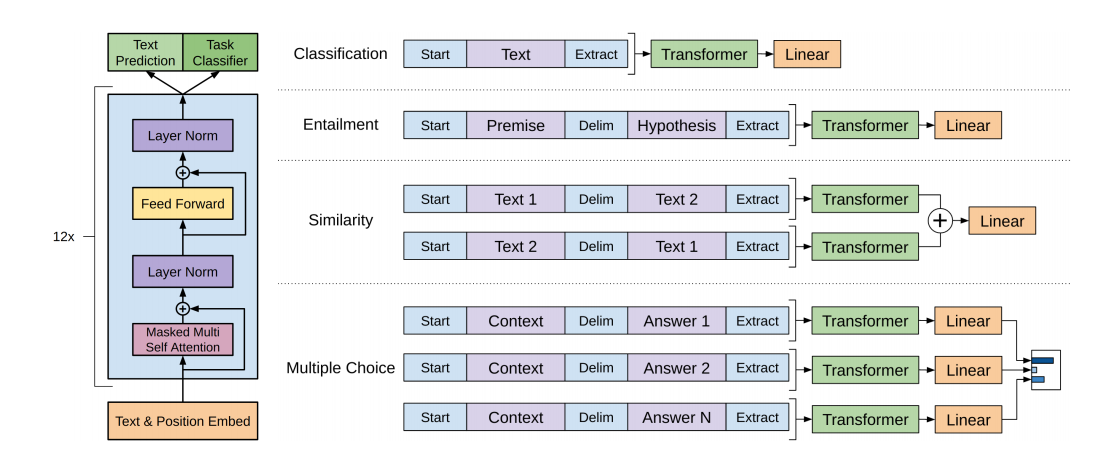
\includegraphics[width = 12cm]{figure/71-gpt}\\
		\citebutton{Source: Radford et al., 2018}{https://openai.com/blog/language-unsupervised/}
	\end{figure}

\vfill

\end{vbframe}

% ------------------------------------------------------------------------------

\begin{vbframe}{Architectural details}

\vfill

	\begin{itemize}
		\item Transformer \textit{decoder} as backbone of the architecture
			\begin{itemize}
				\item 12-layer-decoder with masked self-attention mechanism
				\item Hidden dimension $H = 768$, $A = 12$ Attention heads
				\item BPE vocabulary w/ 40k merges
				\item Learned positional embeddings (as opposed to fixed, sinusoidal ones in the original Transformer)
			\end{itemize}
		\item With $U = (w_{t-k}, \hdots, w_{t-1})$
\begin{align*}
	\vec h_0 &= \vec U \vec W_e + \vec W_p \\
	\vec h_l &= Trafo(\vec h_{l-1}) \forall l \in [1,n]\\
	P(w_t) &= softmax(\vec h_n \vec W_e^\top)
\end{align*}
	\end{itemize}

\vfill

\end{vbframe}

% ------------------------------------------------------------------------------

\begin{vbframe}{Pre-Training GPT}

\vfill

\begin{itemize}
		\item Standard LM objective

\begin{align*}
	L_1(\{w_1, \hdots, w_n\}) = \sum_i \log(P(w_t | w_{t-k}, \hdots, w_{t-1}; \Theta))
\end{align*}
					
					where $\{w_1, \hdots, w_n\}$ is an \textit{unlabeled} sequence of tokens

		\item \textit{Resource:} BooksCorpus 
			\begin{itemize}
				\item > 7k unpublished books from various genres
				\item contains long texts and thus allows learning long range dependencies
			\end{itemize}
\end{itemize}

\vfill

\end{vbframe}

% ------------------------------------------------------------------------------

\begin{vbframe}{Fine-Tuning GPT}

\vfill
			
\begin{itemize}
		\item Linear output layer with softmax activation on top
		\item Auxiliary language modeling objective during fine-tuning\\
					$\rightarrow$ Improves generalization\\
					$\rightarrow$ Accelerates convergence
		\item Task-specific input transformations
					\begin{itemize}
						\item \textit{Entailment:} \\ Concatenation of premise ($p$) \& hypothesis ($h$): $[p; \$; h]$
						\item \textit{Similarity:} Use both orderings and concatenate resulting representations: $[s_1; \$; s_2]$ and $[s_2; \$; s_1]$
						\item \textit{Q\&A and Commensense Reasoning:} \\ Concatenate context ($z$), question ($q$) and each possible answer ($a_k$): $[z; q; \$, a_k]$
					\end{itemize}
		\item Fine-tuning is rather quick, 3 epochs were sufficient
\end{itemize}

\vfill

\end{vbframe}

% ------------------------------------------------------------------------------

\begin{vbframe}{Fine-Tuning GPT}

\vfill

\begin{itemize}
		\item Additional objective:
					\begin{align*}
						L_2(\{w_1, \hdots, w_n\}) = \sum_{x,y} \log(P(y | w_1, \hdots, w_n))
					\end{align*}		
					where 
				\begin{itemize}
					\item $P(y | w_1, \hdots, w_n) = softmax(h_l^m W_y)$ and 
					\item $\{w_1, \hdots, w_n\}$ is a \textit{labeled} sequence of tokens
				\end{itemize}
		\item Combining both objectives: 
					\begin{align*}
						L_3(\{w_1, \hdots, w_n\}) = L_2(\{w_1, \hdots, w_n\}) + \lambda \cdot L_1(\{w_1, \hdots, w_n\})
					\end{align*}
\end{itemize}

\vfill

\end{vbframe}

% ------------------------------------------------------------------------------

\begin{vbframe}{SOTA results}

\vfill

	\textbf{Performance on different benchmarks:}

	\begin{figure}
		\centering
		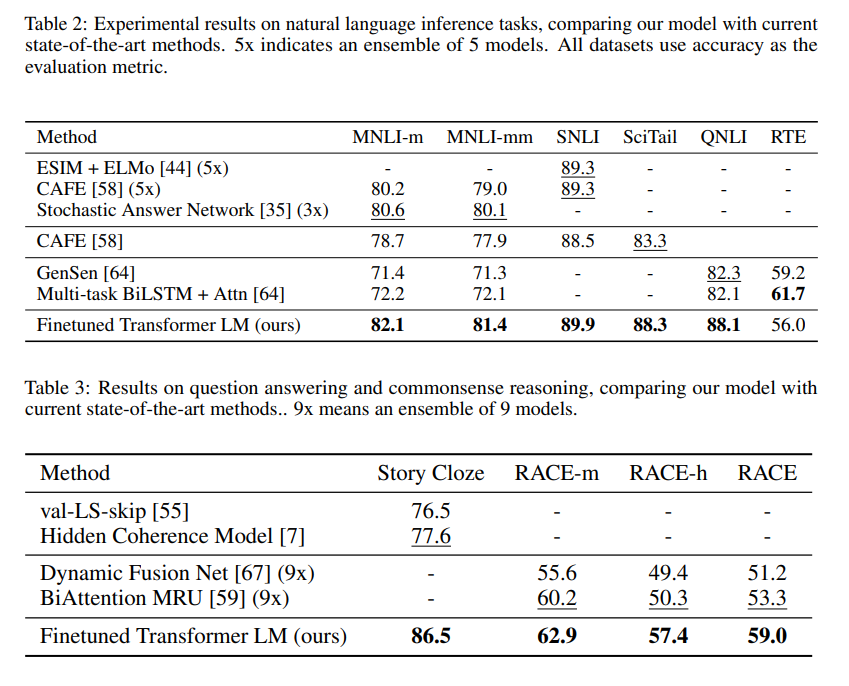
\includegraphics[width = 8cm]{figure/gpt-sota.png}\\ 
		\citebutton{Source: Radford et al., 2018}{https://openai.com/blog/language-unsupervised/}
	\end{figure}

\vfill

\end{vbframe}

% ------------------------------------------------------------------------------

\begin{vbframe}{GPT Parameter Count}

\vfill 

\begin{itemize}
	\item \textbf{We know}: 
		$$n_{layers} = 12; \quad d_{model} = 768; \quad V = 40000; \quad M = 512;$$
	\item \textbf{Also}: 
		$$N_{Decoder} = 12\cdot d_{model}^2 \quad and \quad  N_{Embedding} = \overbrace{V \times d_{model}}^{\text{token embedding}} + \underbrace{M \times d_{model}}_{\text{pos. embedding}}$$
	\end{itemize}

$$
\begin{aligned}
\Rightarrow \quad N_{total} &= n_{layers} \cdot N_{Decoder} + N_{Embedding} \\ 
&= 12\cdot 12\cdot 768^2 + 40000\times 768 + 512\times 768 \\
&= 116,047,872 \approx 117M
\end{aligned}
$$

\vfill
\textbf{Note that $N_{Decoder} = 12\cdot d_{model}^2$ and not $16 \cdot d_{model}^2$ because the Decoder here doesn't do cross attention!}
	
\end{vbframe}

% ------------------------------------------------------------------------------

\endlecture
\end{document}
